\documentclass[BCOR20mm,DIV14,twoside,10pt,headinclude,footexclude,bibtotoc,liststotoc]{scrbook}

\usepackage[utf8]{inputenc}
\usepackage[T1]{fontenc}
\usepackage[ngerman]{babel}
\usepackage[final]{pdfpages}
\usepackage{enumitem}

\titlehead{
\centering
\textbf{Universität Ulm}\\
Fakultät für Ingenieurwissenschaften und Informatik\\
Institut für Organisation und Management von Informationssystemen
}

\subject{
    Masterarbeit\\
    \footnotesize
    im Studiengang Informatik
}

\makeatletter
\title{Steuerung eines Roboters mit Mobiltelefonen} \let\thetitle\@title
\author{Patrick Lutz} \let\theauthor\@author
\newcommand\matrikelnr{752774}
\makeatother

\date{
\footnotesize vorgelegt am\\
\normalsize Dezember 2015
}

\publishers{%
\textbf{Gutachter}\\
Prof. Dr. Stefan Wesner\\
}

% Fonts {{{
\usepackage{helvet}             % Helvetica (eig. Nimbus Sans) Klon
\usepackage[sc]{mathpazo}       % Serif Font fuer Texte
\usepackage{microtype}          % Besseres Kerning, weniger Trennungen
% }}}

% Packages {{{
\usepackage{graphicx}
\usepackage{amsmath, amsthm, amssymb}
\usepackage{listings}
\usepackage{multicol}
\usepackage{booktabs}
\usepackage{url}
\usepackage{ccicons}

\usepackage{natbib}
\setcitestyle{square,numbers,comma,sort}
% }}}

% Bildunterschriften {{{
\usepackage{caption}   % Sans-Serif Font fuer Bildunterschriften
\captionsetup{labelfont={sf,bf},font=sf}
\usepackage[sf,bf,SF]{subfigure}
% }}}

% Bilder {{{
\usepackage{tikz}
% }}}

% Satzspiegel {{{
\renewcommand{\baselinestretch}{1.10}
\setlength{\parindent}{0pt}
\setlength{\parskip}{\baselineskip}
\widowpenalty10000
\clubpenalty10000
% }}}

% Ueberschriftstiefe im TOC
\setcounter{tocdepth}{2}

% Literaturverzeichnis
\bibliographystyle{dinat}

% Kopf- und Fusszeilen {{{
\usepackage{scrpage2}
\pagestyle{scrheadings}
\clearscrheadfoot
\setkomafont{pagehead}{\sffamily}
\automark[section]{chapter}
\ohead{\headmark}
\ofoot{\pagemark}
\setheadsepline{.4pt}
% }}}

% PDF Eigenschaften {{{
\makeatletter
 \usepackage[pdftex,
 	unicode=true,
 	colorlinks=true,
 	linkcolor=black,
 	citecolor=black,
 	urlcolor=black,
 	pdfauthor={\@author}
 ]{hyperref}
\makeatother
% }}}

% Nuetzliche Befehle {{{
\newcommand{\etal}{\emph{et\,al.}}
\newtheorem{defn}{Definition}[chapter]
\newtheorem{thm}{Satz}[section]
% }}}

\hyphenation{%
Fahr-zeug-zu-In-fra-struk-tur-Kom-mu-ni-ka-ti-on
}


\begin{document}

\frontmatter %%%%%%%%%%%%%%%%%%%%%%%%%%%%%%%%%%%%%%%%%%%%%%%%%%%%%%%%%%%%%%%%%%
%\maketitle
\thispagestyle{empty}

\newlength{\backup}
\setlength{\backup}{\headheight}
%\setlength{\headheight}{42mm}


\includegraphics[height=1.8cm]{images/logo_100_sw_bildmarke}
\hfill

\includegraphics[height=1.8cm]{images/logo_100_sw_wortmarke}\\[1em]

{\footnotesize
\hspace*{10.85cm}{\bfseries Fakultät für\\
\hspace*{10.85cm}Ingenieurwissenschaften\\
\hspace*{10.85cm}und Informatik}\\
\hspace*{10.85cm}Institut für Organisation und\\
\hspace*{10.85cm}Management von Informations-
\hspace*{10.85cm}systemen\\[1em]
\hspace*{10.85cm}Januar 2014\\[6em]
}
{\bfseries \huge Title of Thesis\\
}\\[0.5em]
{\large Masterarbeit an der Universität Ulm}\\[1em]
OMI-20XX-M/B-XX\\[4em]

%{\large \bfseries ENTWURF: \today}
%\\[2em]

{\large \bfseries Vorgelegt von:}\\                     
\theauthor \\[2em]
{\large \bfseries Gutachter:}\\                     
Prof. Dr. Stefan Wesner\\
\\[2em]
{\large \bfseries Betreuer:}\\ 
Dr. Lutz Schubert\\


\newpage
\setlength{\headheight}{\backup}


\thispagestyle{empty}

{% impressum
  \newpage
  \small
  \flushleft
  \mbox{}\\\vspace{180mm}

  Fassung \today \\
  {\normalsize \copyright~2014 \theauthor}\\
  %
This work is licensed under the Creative Commons Attribution-NonCommercial-ShareAlike 2.0 License. To view a copy of this license, visit http://creativecommons.org/licenses/by-nc-sa/2.0/de/ or send a letter to Creative Commons, 543 Howard Street, 5th Floor, San Francisco, California, 94105, USA. \\
  %
  Satz: PDF-\LaTeXe
}


\pagestyle{scrheadings}

\clearscrheadfoot
\ohead{\headmark}
\cfoot[\pagemark]{\pagemark}

\chapter*{Abstract}
...

\tableofcontents

\mainmatter %%%%%%%%%%%%%%%%%%%%%%%%%%%%%%%%%%%%%%%%%%%%%%%%%%%%%%%%%%%%%%%%%%%

\chapter{Einleitung}
\label{ch:einleitung}

Die Geschichte der Roboter reicht bis in die Antike zurück. Schon dort gab es erste Versuche mit Automaten, die zum Beispiel Musik spielen sollten oder automatisch Theater spielen konnten. Mit dem Verlust der antiken Kulturen gingen jedoch auch die Kenntnisse über die Automation verloren. Erst im 13. Jahrhundert wurde ein Buch eines arabischen Ingenieurs bis in die westliche Welt bekannt, was Gerüchten zufolge auch Leonardo da Vinci für die Automation inspiriert haben soll. 
Roboter wie wir sie kennen gibt es erst seit Mitte des 20. Jahrhunderts. Der technische Wendepunkt, der mit der Erfindung des Transistors kam, machte es erst möglich, elektrische Schaltungen in einer Größe zu fertigen, die für Roboter notwendig ist. Seit diesem Zeitpunkt liegt ein wertvoller und nicht mehr wegzudenkender Industriezweig auf dem Gebiet der Robotik. Mit dem Einstieg der Robotik in die Industrie wurde die Produktion um ein vielfaches schneller und präziser, als sie von Menschenhand je vorgenommen werden könnte. Auch in Bereichen oder Umgebungen, die für Menschen lebensgefährlich oder ohnehin lebensunmöglich sind, spielen Roboter eine bedeutende Rolle. Ein Beispiel hierfür ist der Mars-Rover. Der Mars-Rover ist ferngesteuertes Fahrzeug, welcher für die Marsforschung verwendet wird und größten Teils von der Erde aus gesteuert wird. Wie die meisten ferngesteuerten Fahrzeuge ist er mit einer Vielzahl von Sensoren und Werkzeugen ausgestattet. 

Seit Ende der 90-er Jahre gibt es einen weltweiten Wettbewerb namens RoboCup. Bei RoboCup geht es darum, ein Fussballspiel von Robotern austragen zu lassen. Diese Bachelorarbeit beschäftigt sich ebenfalls mit dem Thema der Steuerung von mobilen Robotern mit dem Ziel, ein Roboter-Fussballspiel zu ermöglichen. Im Gegensatz zum RoboCup, bei dem die Roboter entweder autonom, oder von einem zentralen Computer gesteuert werden, der mittels einer Kamera über dem Spielfeld die Bewegungen und Situationen erfasst, wird in dieser Bachelorarbeit die Steuerung der Roboter vom Menschen übernommen. Auf einer Tischplatte in der Universität sollen zwei Roboter platziert werden. An den beiden Enden der Tischplatte werden Tore montiert, ähnlich wie man es beim Tischfussball kennt. Mithilfe von mobilen Endgeräten sollen nun die Roboter angesteuert werden können und ein Zwei-Spieler Fussballspiel ermöglicht werden. Die Roboter verfügen über einen Schussapparat, der es möglich macht den Ball zu beschleunigen. Sobald der Ball in ein Tor befördert wurde, wird ein Tor automatisch erkannt und auf den mobilen Endgeräten, welche die Steuercontroller bilden, angezeigt. Diese Steuercontroller können entweder ein Android-Gerät oder jedes beliebige andere Gerät sein, das über eine Tastatur und einen Webbrowser verfügt. Über diese Steuercontroller ist es möglich die Roboter zu navigieren und einen Schuss zu tätigen. Hierfür werden verschiedene Steuerarten bereitgestellt. 
Die Roboter bewegen sich vollkommen kabellos, was die Verwendung eines Akkus notwendig macht. Sobald der Akku einen Mindestprozentsatz unterschreitet, wird automatisch die Ladestation angefahren, damit sich der Akku des Roboters selbstständig, also ohne menschliches Eingreifen, lädt.
Die Fertigung und Implementierung der Roboter ist Teil einer anderen Bachelorarbeit, auf die hier nur Oberflächlich eingegangen wird.               

% hier kommt noch ein kurzer überblick über die arbeit, welche kapitel folgen und was in welchen kapiteln ungefähr beschrieben wird




\section{Anforderungen}
Das Ziel der Bachelorarbeit ist es, ein Fussballspiel für zwei Spieler zu realisieren. Hierfür werden zwei Roboter auf einem begrenzten Spielfeld positioniert. Jeweils am Rand des Spielfelds wird ein Tor montiert, in das der Ball befördert werden soll. Mittels mobilen Endgeräten und herkömmlichen PCs soll es möglich sein, die Steuerung über einen der Roboter zu übernehmen. Sobald beide Roboter mit einem Steuergerät verbunden sind, soll ein Spiel gestartet werden und die Torerkennung funktionieren. Das bedeutet, sobald ein Spieler ein Tor erzielt hat, erkennt das System dieses und erhöht den Spielstand dementsprechend. Mittels einer Kamera, die auf den Robotern montiert ist, soll eine Videoübertragung aus Sicht der Roboter stattfinden. Dadurch soll es auch möglich sein, die Roboter zu steuern, ohne sich in Sichtkontakt mit den Robotern zu befinden. Da die Roboter über einen Akku verfügen, soll die Kommunikation kabellos erfolgen, damit ein freies Fahren der Roboter sichergestellt ist. Weil der Akku eine begrenzte Kapazität hat, soll der Roboter bei niedrigem Akkustand selbstständig die Ladevorrichtung anfahren und während der Ladezeit keine Steuerbefehle annehmen. Aufgrund der Interaktion mit menschlichen Benutzern, ist es wichtig, dass der Roboter eine möglichst rechtzeitige Steuerung darstellt, um Verzögerungen und die dadurch entstehende Unkontrollierbarkeit zu vermeiden.


\section{Schnittstelle zum Roboter}
\label{sec:schnittstelle}
                                                                                                                                                                                                                                                                                                                                                                                                                                                                                                                                                                                                                                                                                                                                                                                                                                                                                                                                                                                                                                                                                                                                                                                                                                                                                                                                                                                                                                                                                                                                                                                                                                                                                                                                                                                                                                                                                                                                                                                                                                                                                                                                                                                                                                                                                                                                                                                                                                                                                                                                                                                                                                                                                                                                                                                                                                                                                                                                                                                                                                                                                                                                                                                                                                                                                                                                                                                                                                                                                                                                                                                                                                                                                                                                                                                                                                                          
                                                                                                                                                                                                                                                                                                                                                                                                                                                                                                                                                                                                                                                                                                                                                                                                                                                                                                                                                                                                                                                                                                                                                                                                                                                                                                                                                                                                                                                                                                                                                                                                                                                                                                                                                                                                                                                                                                                                                                                                                                                                                                                                                                                                                                                                                                                                                                                                                                                                                                                                                                                                                                                                                                                                                                                                                                                                                                                                                                                                                                                                                                                                                                                                                                                                                                                                                                                                                                                                                                                                                                                                                                                                                                                                                                                                                                                          
                                                                                                                                                                                                                                                                                                                                                                                                                                                                                                                                                                                                                                                                                                                                                                                                                                                                                                                                                                                                                                                                                                                                                                                                                                                                                                                                                                                                                                                                                                                                                                                                                                                                                                                                                                                                                                                                                                                                                                                                                                                                                                                                                                                                                                                                                                                                                                                                                                                                                                                                                                                                                                                                                                                                                                                                                                                                                                                                                                                                                                                                                                                                                                                                                                                                                                                                                                                                                                                                                                                                                                                                                                                                                                                                                                                                                                                                                                                                                                                                                                                                                                                                                                                                                                                                                                                                                                                                                                                                                                                                                                                                                                                                                                                                                                                                                                                                                                
% ...

\chapter{Grundlagen}
\label{ch:Grundlagen}


UDP

Beim User Datagram Protocol handelt es sich um ein verbindungsloses und in jeglicher Hinsicht ungeschütztes Protokoll, das auf der Transportebene (Schicht 4 im OSI-Schichtenmodell) arbeitet. Es bestehen keinerlei Mechanismen, die das korrekte Übertragen von Paketen gewährleisten. Hierzu zählen:

\begin{description}
	\item[Sicherheit] Die Sicherheit, dass Pakete überhaupt ankommen
	\item[Reihenfolge] Die Reihenfolge, in der Pakete ankommen
	\item[FlowControl] Ein Überlaufschutz des Empfängerspeichers (FlowControl)
	\item[CongestionControl] Stauvermeidung in der Übertragungskette (CongestionControl)
	\item[Angriffe] Schutz gegen Paketmanipulation von dritten
\end{description}

\begin{figure}
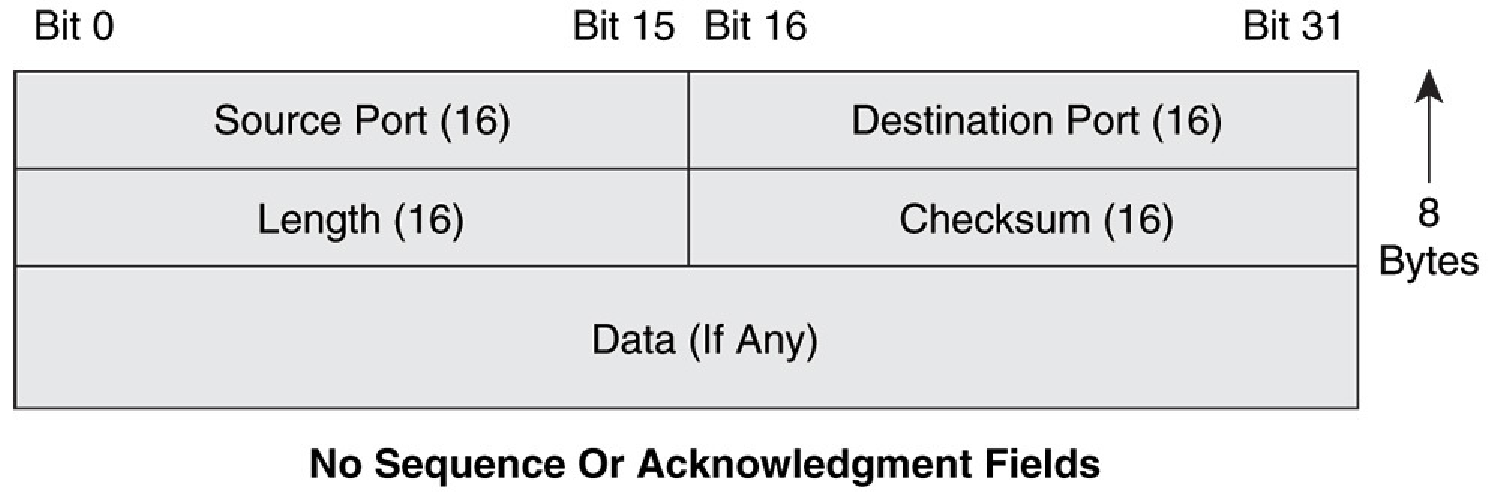
\includegraphics[width=\textwidth]{images/UDP_header.pdf}
\caption{UDP Header}
\label{fig:udp_header}
\end{figure}

Ein UDP Header besteht aus 8 Byte. Mit diesen 8 Byte werden lediglich Source-Port, Destination-Port, Länge und die Checksumme übertragen. Dieser vergleichsweise kleine Header (vgl. TCP mit etwa 20 Byte), führt zu einem geringen Overhead während der Übertragung, auch bei kleinen Paketen. Nachdem ein Paket gesendet wurde erfolgt keine Bestätigung des Pakets vom Empfänger. Durch diesen Uni-Direktionalen Sendevorgang entsteht wenig Traffic im Netzwerk. Falls gewisse Sicherheitsmechanismen gewünscht sind, müssen diese in höheren Schichten implementiert werden. \\
Aufgrund dieser Eigenschaften wird UDP in Bereichen eingesetzt, in denen es auf hohe Übertragungsgeschwindigkeit ankommt und eventuelle Paketverluste zu verkraften sind, bzw. von höheren Schichten aufgelöst werden.




\newpage


TCP

Beim Transmission Control Protocol handelt es sich um ein verbindungsorientiertes paketvermittelndes Protokoll. Mithilfe verschiedener Mechanismen wird sichergestellt, dass Pakete in der richtigen Reihenfolge ankommen, es zu keinen Staus kommt und dass Netzwerkknoten nicht überlaufen. Dadurch, dass das Protokoll verbindungsorientiert arbeitet, können beide Teilnehmer der Verbindung Daten ohne Anfragen senden. 

\begin{figure}
	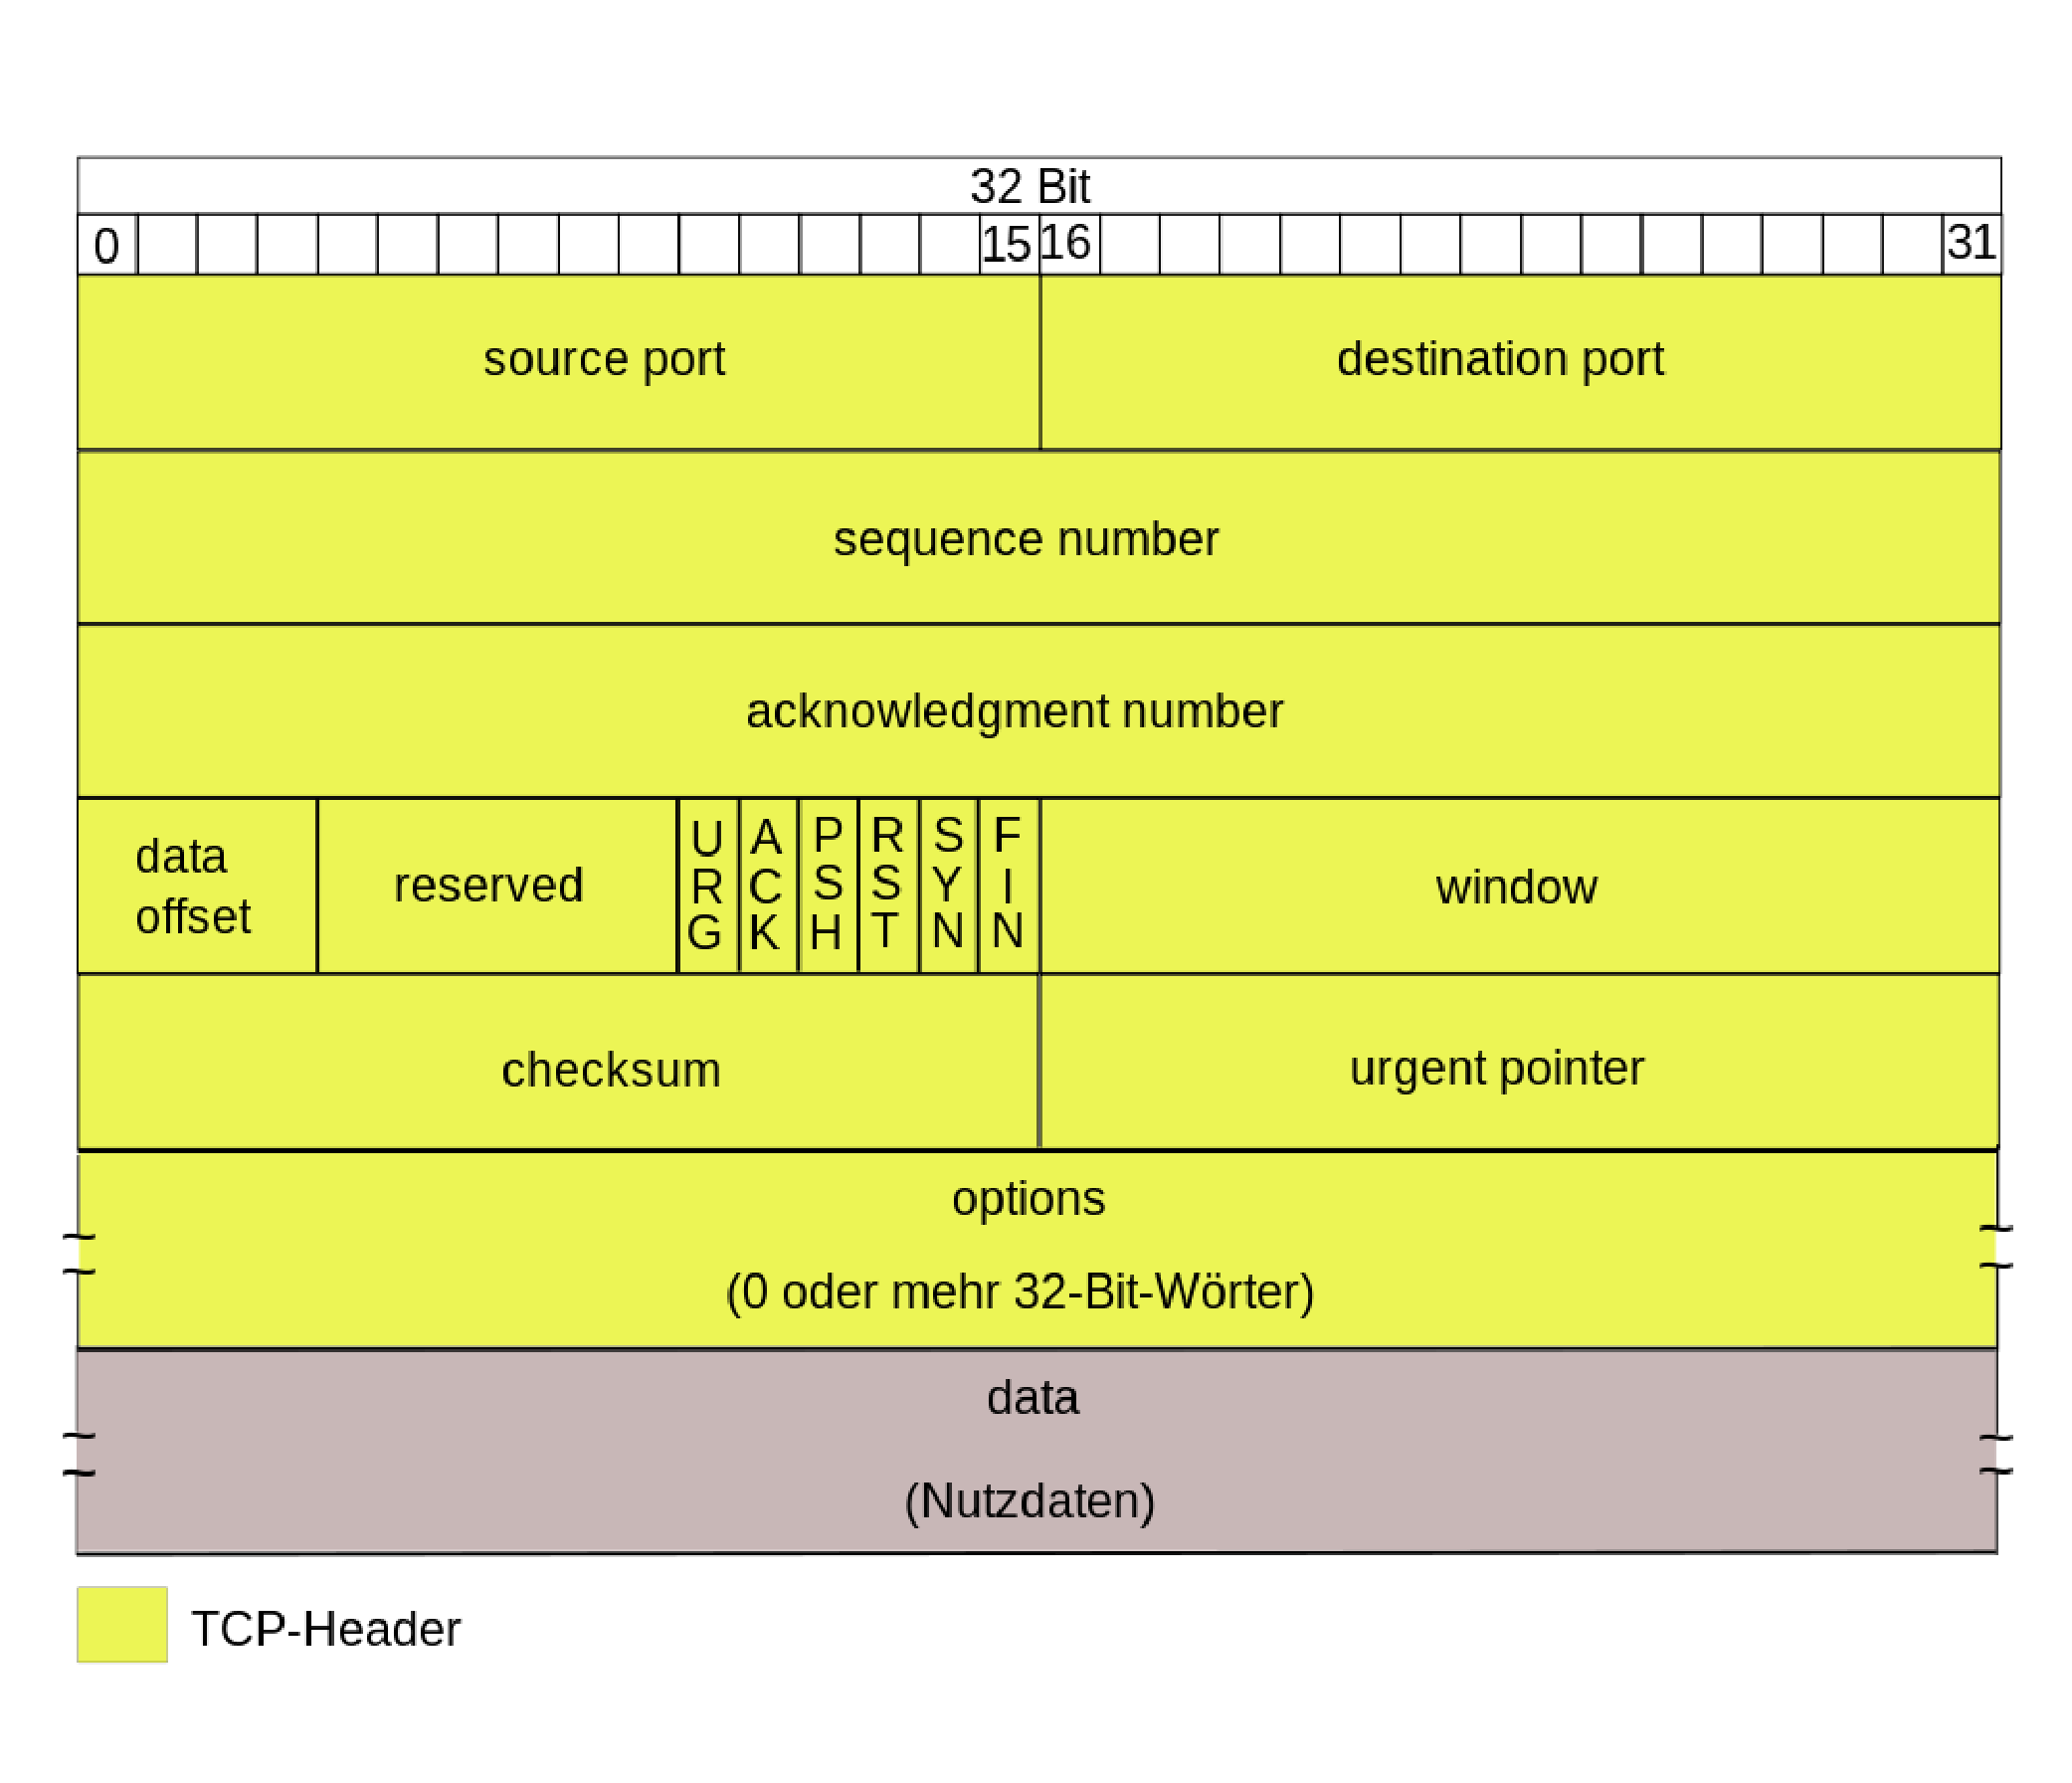
\includegraphics[width=\textwidth]{images/TCP_header.pdf}
	\caption{TCP Header}
	\label{fig:tcp_header}
\end{figure}

Durch den größeren Header und dem größeren Traffic, der das Protokoll verursacht, wird TCP für Anwendungen verwendet, bei denen ein Paketverlust ausgeschlossen werden soll, dafür aber eine etwas höhere Latenz in Kauf genommen werden kann. 
Die Verbindung wird über einen 3-Wege-Handshake hergestellt. Hierbei sendet ein Teilnehmer eine Anfrage (syn), diese wird bestätigt (syn ack) woraufhin die Bestätigung erneut bestätigt wird. In diesem dritten Schritt werden meist bereits die ersten Nutzdaten mitgesendet.
\begin{figure}
	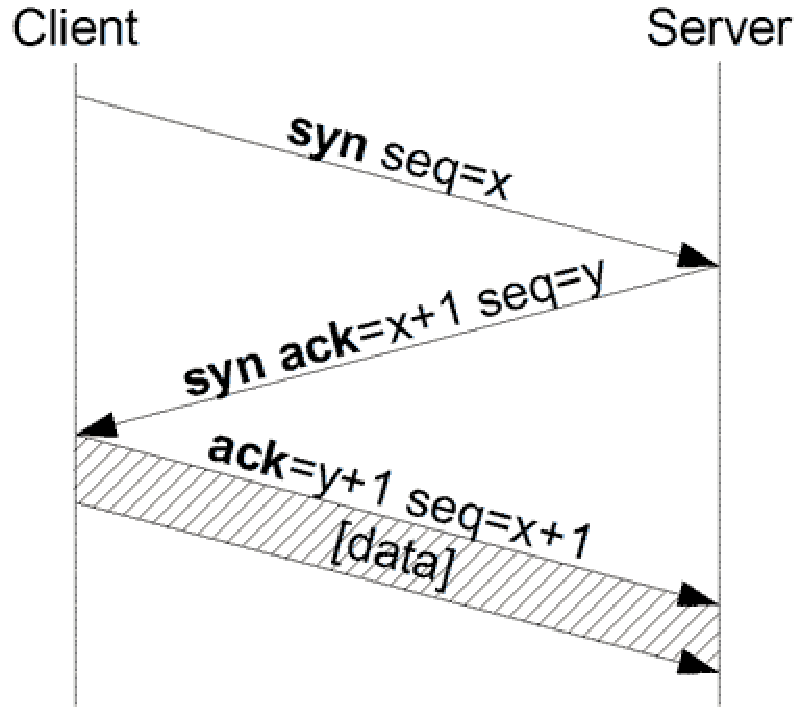
\includegraphics[width=\textwidth]{images/TCP_3wayhandshake.pdf}
	\caption{TCP 3-Wege-Handshake}
	\label{fig:tcp_3wayhandshake}
\end{figure}

Mithilfe von geordneten Sequenznummern und Acknowledgments werden alle empfangene Pakete bestätigt. Durch das Fehlen einer Sequenznummer erkennt der Empfänger den Verlust eines Pakets und teilt daraufhin dem Sender mit, dass es nicht angekommen ist. Für den Fall eines Verlusts des Acknowledgments, hat der Sender einen Timer, welcher nach einiger Zeit eine Retransmission des Pakets veranlasst, sofern kein Acknowledgment ankommen sollte.




HTTP

Das Hypertext Transfer Protocol ist ein zustandsloses Datenübertragungsprotokoll, das auf der Anwendungsschicht arbeitet. Am meisten wird das Protokoll für den Aufbau von Internetseiten verwendet, also von einem Webbrowser, jedoch ist das Aufgabenfeld nicht darauf beschränkt.

HTTP arbeitet mittels zwei Befehlsarten, dem Request und dem Response. Möchte ein Browser eine Datei von einem Server laden, so sendet er einen Request mit dem Namen der Datei. \\
Die möglichen Befehle sind: 
\begin{description}
	\item[GET] fordert eine Ressource auf dem Server an
	\item[POST] sendet Daten zur weiteren Verarbeitung zum Server
	\item[HEAD] fordert lediglich den HEADER eines Responses an, der auf einen GET-Request folgend würde
	\item[PUT] lädt eine Ressource auf den Server
	\item[DELETE] löscht eine Ressource auf dem Server (Wird kaum verwendet)
	\item[TRACE] sendet die Anfrage, so wie sie empfangen wurde zurück
	\item[OPTIONS] liefert eine Liste mit den vom Server unterstützten Optionen
	\item[CONNECT] wird für SSL-Tunneling verwendet
\end{description} Nachdem der Request beim Server eingegangen ist und verarbeitet wurde, sendet er einen Response. In diesem Response sind Informationen über Server und Datei enthalten, sowie die Nutzdaten, also die angefragte Datei. In Abbildung \ref{fig:http_request_response} ist eine solche Kommunikation dargestellt.
-- 
\begin{figure}
	\includegraphics[width=\textwidth]{images/http_request_response.pdf}
	\caption{HTTP Kommunikation}
	\label{fig:http_request_response}
\end{figure}



WebSockets

Das WebSocket-Protokoll ist ein Netzwerkprotokoll, das auf TCP und HTTP basiert. In diesem Protokoll ist es möglich, eine bidirektionale Verbindung zwischen einer Webanwendung und einem WebSocket-Server herzustellen. Im Gegensatz zu reinem HTTP ist es hierbei möglich, dass der Server ohne einen vorhergehenden Request des Clients, Daten an den Client sendet. Lediglich den Verbindungsaufbau muss der Client initiieren. Dies wird realisiert, indem die TCP-Verbindung nach dem Verbindungsaufbau nicht sofort geschlossen wird. 
Eine WebSocket URL wird über die beiden Schemata wss und ws definiert, was für verschlüsselte und unverschlüsselte Verbindungen steht.

Der Verbindungsaufbau funktioniert über einen Handshake, der wie in HTTP üblich über einen Request und anschließenden Response erreicht wird. Aufgrund der Tatsache, dass die HTTP-Header nur beim Verbindungsaufbau gesendet werden und dadurch der Traffic durch den HTTP-Header gering ist, wird das Protokoll hauptsächlich von Anwendungen verwendet, die regelmäßige Kommunikation zwischen Client und Server verlangen, wie zum Beispiel Online-Spiele.



Jetty Webserver

Jetty ist eine Java-Implementierung eines Webservers. Durch seine geringe Größe ist es leicht, ihn in andere Software zu integrieren. Außerdem unterstützt Jetty die Möglichkeit WebSockets aufzubauen.
% ...


\backmatter %%%%%%%%%%%%%%%%%%%%%%%%%%%%%%%%%%%%%%%%%%%%%%%%%%%%%%%%%%%%%%%%%%%

\null\cleardoublepage

%\cite{*}
%\bibliographystyle{dinat} %first referenced
\bibliography{../literature/references.bib}

\cleardoublepage
\clearscrheadfoot
\ihead{Name: \theauthor}
\ohead{Matrikelnummer: \matrikelnr}
\cfoot{\pagemark}

\minisec{Erklärung}

Ich, \theauthor, Matrikelnummer \matrikelnr, erkläre, dass ich die Arbeit
selbständig verfasst und keine anderen als die angegebenen Quellen und
Hilfsmittel verwendet habe.

\vspace{2cm}

Ulm, den \dotfill

\hspace{10cm} {\footnotesize \theauthor}

\end{document}